\section{Case Study: Introducing the MockingJay Process Injection Attacks}

In our review of one technique used by malware groups, we now ask how a CISO in a modern organisation can stay ahead of the curve,
have an realistic appraisal of the threats their organisation might face, and develop a resilient cybersecurity infrastructure.

Our hyperthetical CISO has been active in putting in place an XDR system that has reduced manual processes to patch individual cybersecurity
applications, leveraged the vendor's expertise to configure the monitoring of data across endpoints, servers, cloud networks and Security
information and event management (SEIM) systems.

Our enlightened CISO has empowered his team team to research ways to improve cybersecurity, and looks foward to using their insights to engage with
senior stakeholds within the organisation, and to regularly brief the board on operation risks and mitigation plans.  

One of the team security engineers has come across a new potential exploit and has asked to produce this case study for the CISO and his team.  The
Mockingjay attack \autocite{Peixoto:2023} is a real and novel process injection attack created by Security Joes, a
``multi-layered MDR \& incident response company'' based in Tel Aviv.

\subsection{Introduction}


\textbf{Key Problems}:

\begin{enumerate}
\item A new process injection attack has been identified by Securities Joe.  The exploit circumvents the allocation
  and permission APIs that most EDR systems monitor.  It  does this by using existing RWX code sections without invoking
  new threads.
\item Our systems may be vulnerable to this attack which could allow a Windows executable to self injection or remote injection.
\item Recently Citrix has reported vulnerabilities in their NetScaler Application Delivery Controller (ADC) and Gateway products that
  could allow:
  \begin{itemize}
  \item \citetitle{CVE-2023-3467} \autocite{CVE-2023-3467}.
  \item \citetitle{CVE-2023-3519} \autocite{CVE-2023-3519}.
  \item \citetitle{CVE-2023-4966} \autocite{CVE-2023-4966}.
  \end{itemize}
\item The Cybersecurity and Infrastructure Security Agency (CISA) has reported that the malware group LockBit \autocite{CISA:2023a} has
  been found to be actively exploiting CVE-2023-4966 to obtain initial access to Boeing Distribution Inc. \autocite{CISA:2023b}.
\end{enumerate}

Our organisation should be prepared for similar attacks and group should review our cyber-defences in light of this information.
As always, we should seek to prevent any successful attack, but also improve our cyber-resilience in the face of a sucessful breach.

This case study will:
\begin{enumerate}
\item Review the salient points of the new attack vector, how it may evade our XDR system and how we may identify an attack.
\item Understand ransomware threat actors such as LockBit and how we can detect and respond to ransomware.
\item Prepare a set of recommendations in line with our Cyber-Security Framework (CSF) \autocite{NIST:2018}.
\end{enumerate}


%\subsection{Real-world examples of malware employing process injection on Windows}
\subsection{Context: Detailed Analysis of New Process Injection Attack}

Attackers could exploit the Mockingjay technique to circumvent XDR process monitoring and anti-virus sofware by avoiding
common system API calls used by malware.  

The security report was able to demonstrate:

\begin{enumerate}
\item Self-injection
\item Remote process injection: injected a shellcode into `ssh.exe` in the
\end{enumerate}

\subsection{Alternatives: How Attack could Evade XDR}

The first line of our defense of an attack based on the Mockingjay process injection technique will be our XDR system.

Using `Lifecycle of a Ransomeware Incident` produced by \autocite{Certnz:2021} and the modus-operandi of the LockBit
group \autocite{CISA:2023}, we should anticipate:

\begin{enumerate}
\item Direct attack through our application gateway (Intenet-exposed Service).
\item Phishing attack through email.
\end{enumerate}

If either of these two approaches are successful, 

\begin{figure}[ht]
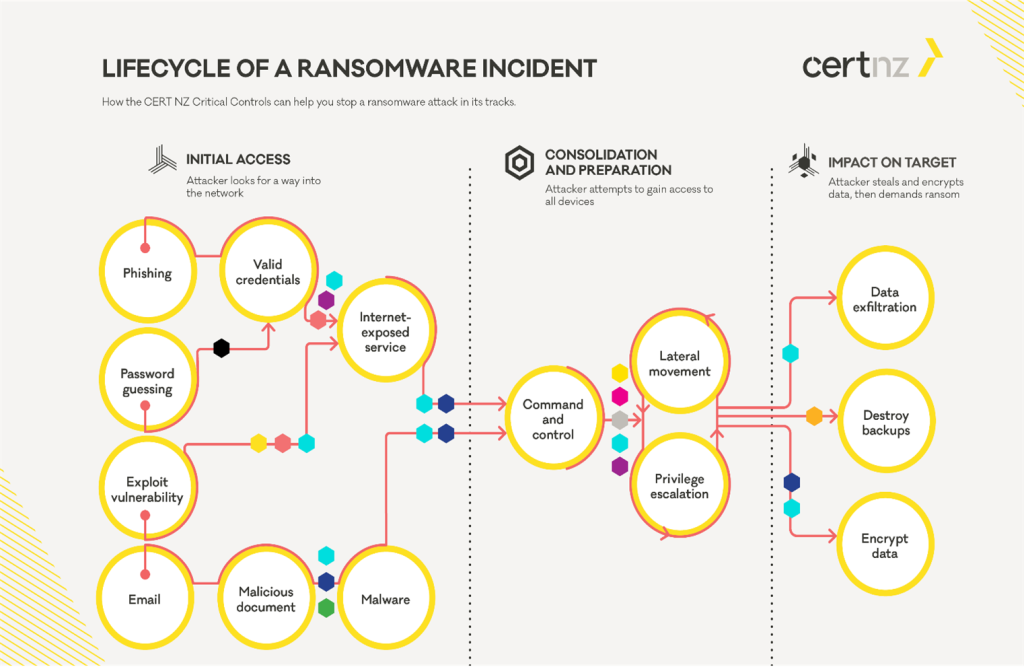
\includegraphics[scale=0.55]{certnz_aa23-165a.png}
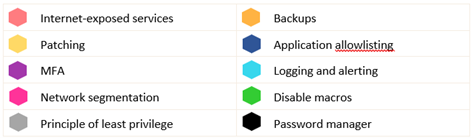
\includegraphics[scale=0.6]{certnz_aa23-165b.png}
\caption{Ransomeware Layered Mitigations \autocite{Certnz:2021}}
\end{figure}

\pagebreak

%\subsection{Analysis of the impact and consequences of these incidents}
\subsection{Proposed Solution: Assessing and Improving Cybersecurity Measures}

As Security Joes is a security system vendor, the report itself lists a number of ways that the attack could be detected. At
the first instance, we should be talking to our XDR vendor to ensure we have the functionality to automate these steps.  At
the very least we need to be able to perform ad-hoc scans across our infrastructure and windows systems to flag the following:

\begin{enumerate}
  \item point a:
\end{enumerate}


\subsection{Recommendations}

Our organisation is committed to the continud review of new attacks and actively researches the possible impact of reported attacks.
This active engagement with the cybersecurity community and our vendors allows us to adapt quickly to changes in the threat landscape.

For this case study, we recommend the following actions under each of the NIST CSF fuctions:

\begin{itemize}
\item Identify: Ensure all systems are patched for the CVEs identified and engage with our XDR vendor to respond to this new threat.
\item Protect: review XDR solutions are monitoring log files to detect encryption; use technique to find vulnerable exes and block them (eg. visual studio ssh exfiltration block known malicios systes
\item Detect: Develop a Mockingjay red-team exercise against our XDR; test for the detection of the loading of NTDLL.dll from disk.
\item Respond: Ensure that our organisation is able to report to all relevant authorities  and abide to our legal responsibilities for disclosuress
\item Recover: review perform disaster recover tests to restore systems from backups and that backups are immutable 
\end{itemize}




